\chapter{Metodología y materiales}
\label{ch:inicioIR}

En este capítulo se exponen las fases en las que se va a realizar el estudio, los datos recopilados y el entorno experimental que se utilizan para el desarrollo del proyecto.
\section{Metodología}

La metodología seguida en este trabajo se ha diseñado para abordar de forma sistemática el estudio, adaptación y evaluación de modelos de lenguaje en lenguas minoritarias de España. El proceso es un pipeline que se estructura en cinco fases consecutivas, cada una con objetivos y actividades claramente definidos, que permiten avanzar desde la exploración inicial del estado del arte hasta la obtención de un modelo ajustado y su evaluación comparativa.

\subsection*{Fase 1: Exploración de modelos existentes}
En esta primera fase se analizan los modelos de lenguaje disponibles que puedan servir como punto de partida para el estudio. Se revisan sus arquitecturas, tamaños, capacidades multilingües y rendimiento en las lenguas cooficiales, apoyándose en recursos como la \textit{leaderboard} de SomosNLP. El objetivo es identificar modelos representativos en distintos rangos de parámetros y con enfoques arquitectónicos diversos, que permitan comprender las limitaciones actuales en lenguas de bajo recurso.

\subsection*{Fase 2: Definición de métricas y tareas de evaluación}
Una vez identificados los modelos candidatos, se diseña un conjunto de métricas y tareas que permitan evaluar su rendimiento de forma homogénea. Se seleccionan tareas relevantes para lenguas minoritarias, como traducción, corrección gramatical o análisis de interferencias lingüísticas. Para cada tarea se establecen métricas cuantitativas (BLEU, chrF++, tasas de error) y criterios cualitativos, garantizando una evaluación reproducible y comparable entre modelos.

\subsection*{Fase 3: Selección y preparación del modelo a adaptar}
Tras la evaluación preliminar, se selecciona el modelo más adecuado para ser adaptado mediante técnicas de \textit{fine-tuning} eficiente. En esta fase se realiza la preparación del modelo base, la configuración de los parámetros de entrenamiento, la integración del QLoRA y la configuración de los hiperparámetros. Asimismo, se lleva a cabo la limpieza, normalización y alineación de los conjuntos de datos necesarios para el entrenamiento del modelo en las lenguas objetivo.

\subsection*{Fase 4: Entrenamiento y análisis del modelo adaptado}
En esta fase se entrena el modelo seleccionado utilizando los datos preparados y la configuración definida. Se monitoriza el proceso de entrenamiento, analizando la estabilidad, la convergencia y el impacto del QLoRA. Además, se documentan las decisiones tomadas durante el proceso y se evalúan los primeros resultados para detectar posibles problemas o mejoras necesarias.

\subsection*{Fase 5: Evaluación final y comparativa}
Finalmente, el modelo adaptado se evalúa utilizando las métricas y tareas definidas en la Fase 2. Se comparan sus resultados con los obtenidos por los modelos analizados en la Fase 1, permitiendo determinar si la adaptación ha mejorado el rendimiento en las lenguas minoritarias. Esta fase incluye tanto un análisis cuantitativo como cualitativo, así como una discusión de las limitaciones y del impacto real de la adaptación realizada.
\\
\\
Un gráfico que muestra la metodología seguida y su flujo secuencial, se puede observar en la Figura \ref{fig:metodologia-trabajo}.

\begin{figure}[H]
    \centering
    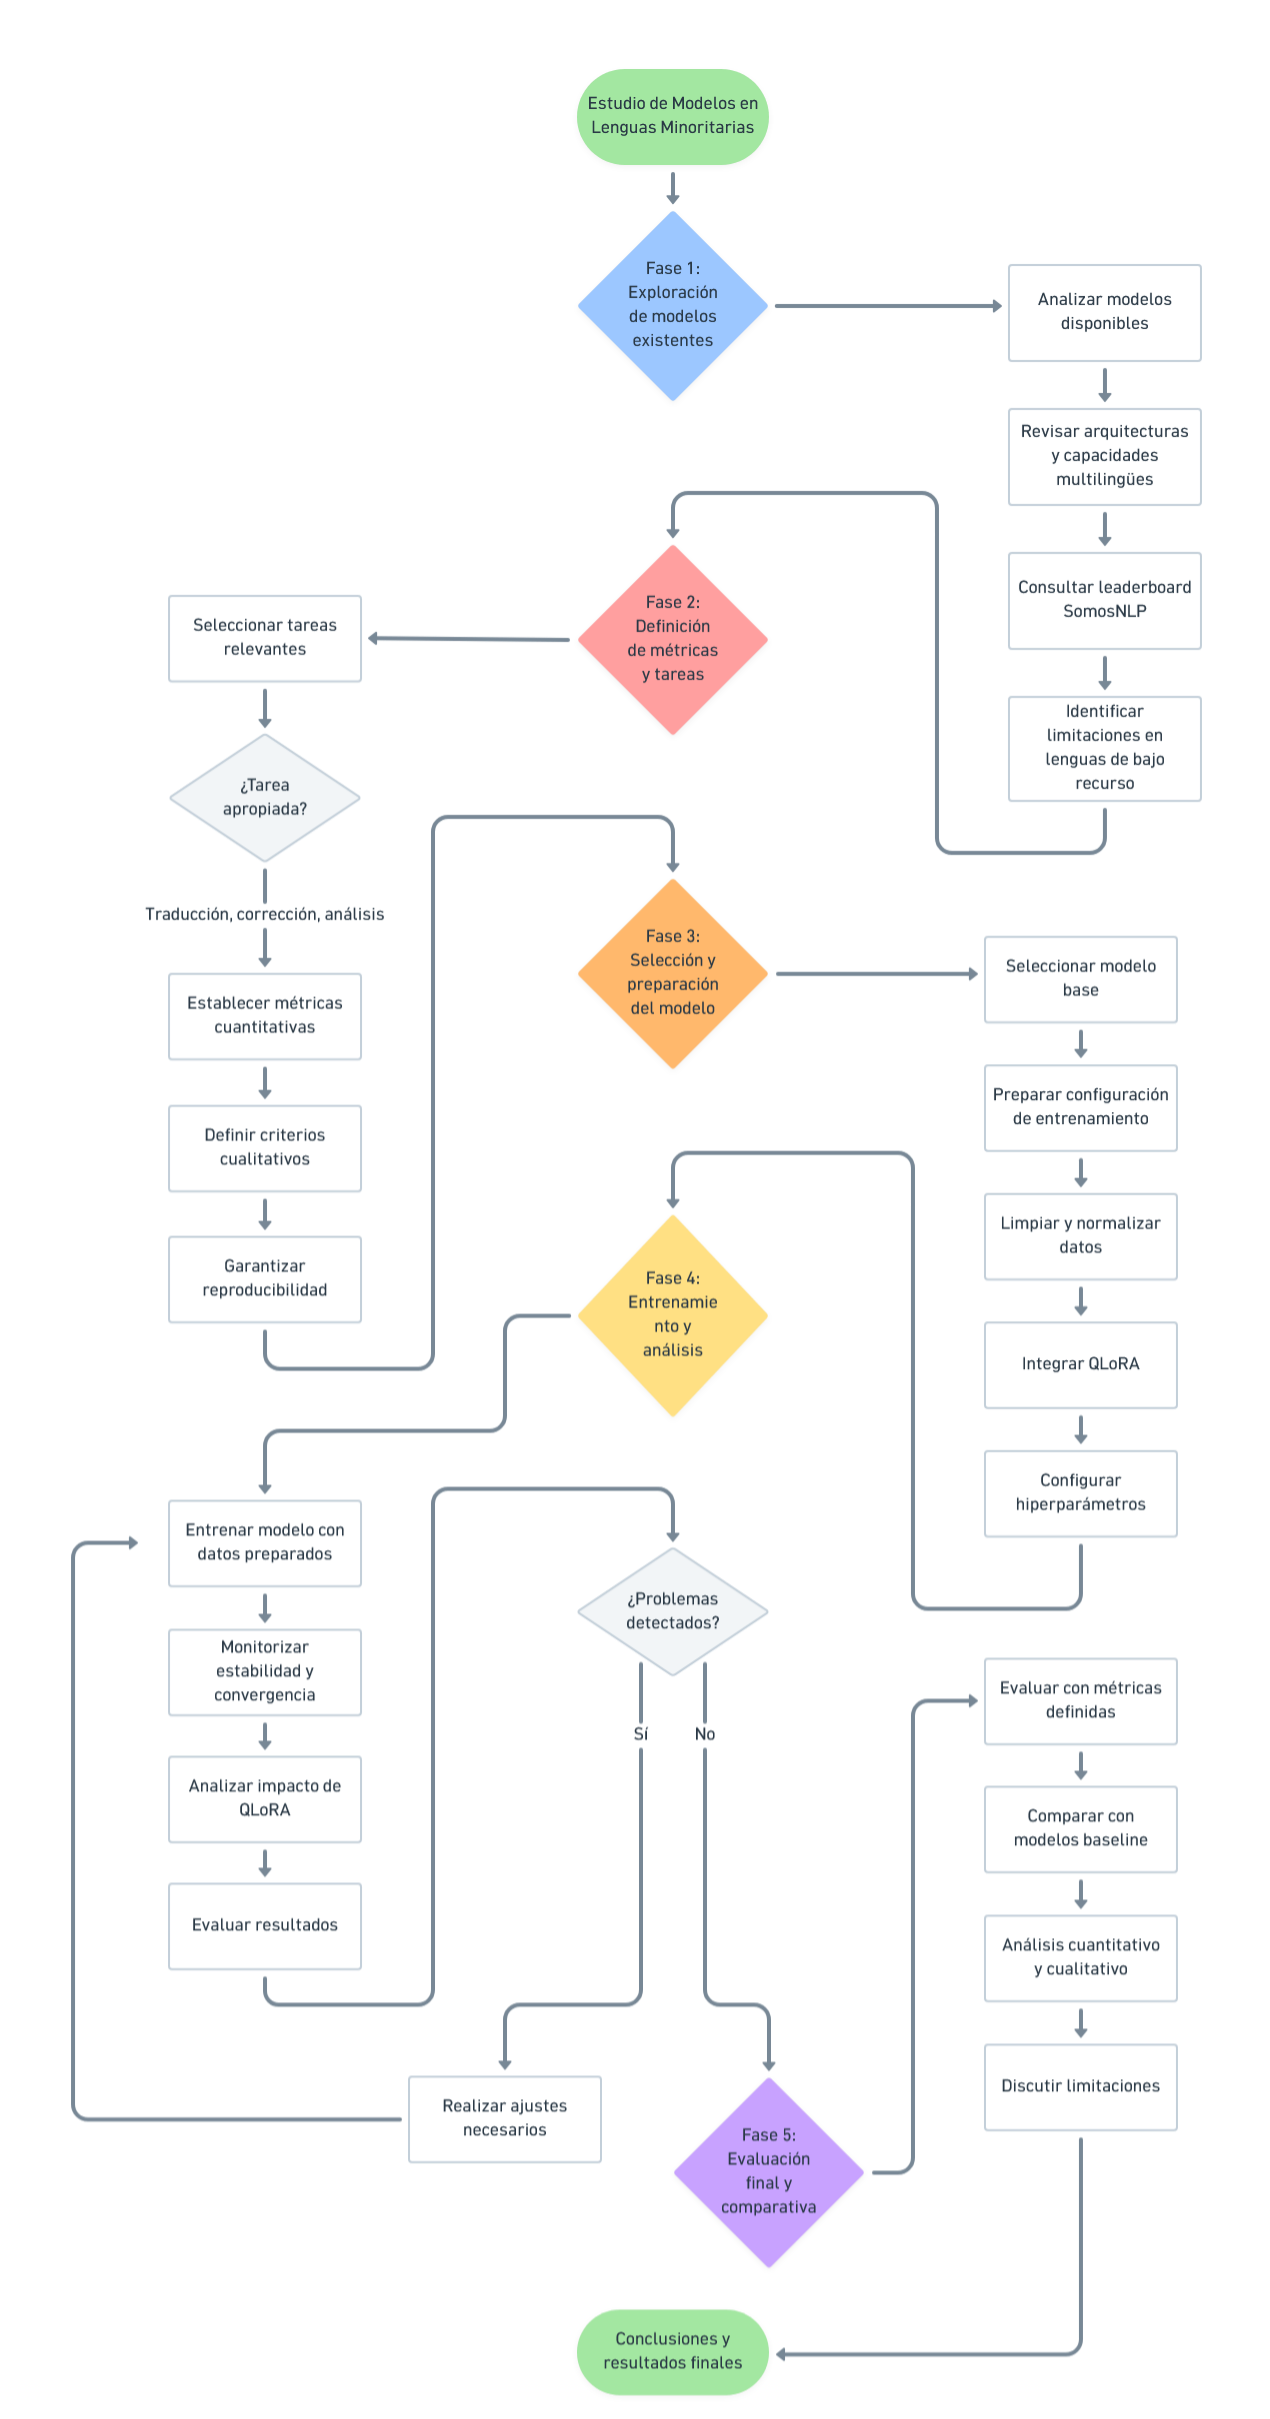
\includegraphics[width=0.8\textwidth]{figures/MetodologíaV2.png}    
    \caption{\label{fig:metodologia-trabajo} Resumen visual de la metodología empleada. De creación propia.}
\end{figure}


\section{Materiales}

\subsection{Conjuntos de datos}
\label{conjuntos-de-datos}
\subsubsection{Proceso de exploración}
Se ha comenzado revisando los datasets utilizados por Alia, analizando los idiomas que incluyen y el número de frases disponibles en cada uno. 
Posteriormente se han buscado otras fuentes de datos, entre las cuales destaca OPUS, que es especialmente grande. 

Todas estas fuentes permiten descargar y utilizar los datos con facilidad, aunque algunos corpus son muy voluminosos, quizá demasiado para ciertos usos.

\subsubsection{Datasets previamente encontrados}

Alia, la infraestructura pública de IA en castellano y lenguas cooficiales, ofrece conjuntos de datos de texto, voz y traducción automática. Es un recurso útil tanto para obtener datos como para comparar resultados \cite{ALIA2025}.

Otra gran plataforma donde se pueden encontrar varios conjuntos de datos es \textbf{OPUS}. OPUS reúne y distribuye corpus paralelos multilingües de acceso abierto. Su objetivo es facilitar la investigación en traducción automática, alineación de textos y aprendizaje de modelos multilingües. Los datos provienen de múltiples fuentes (como subtítulos, documentos oficiales o la Wikipedia). Se utilizarán los datos de esta web para el asturiano y el aranés, que no cuentan con un conjunto de datos grande ya creado \cite{tiedemann-2012-parallel}.

Para el \textbf{gallego} se encontró un dataset de más de 2 mil millones de palabras. Este corpus se nutre de libros, enciclopedias, datos gubernamentales, prensa, artículos de investigación, webs públicas, Wikipedia, corpus de traducción y otros web crawls \cite{CorpusNOS-GL}.

Por otro lado, se encuentra el proyecto LiLowLa \cite{LiLowLa2022} de la Universidad de Alicante. El objetivo de este proyecto \textit{(Lightweight neural translation technologies for low-resource languages)} es mejorar el rendimiento de la traducción automática neuronal y de las memorias de traducción en pares de lenguas con escasos recursos. Incluye un dataset con texto en aragonés, aranés, asturiano y valenciano \cite{perez-ortiz-etal-2024-expanding}.

También se incluirán los datos de \textbf{Tatoeba}. Aunque el número de frases en asturiano y aranés es reducido, resulta una fuente útil para ampliar la cobertura y enriquecer los conjuntos de datos ya mencionados \cite{Tatoeba2025}.

Finalmente, se pueden extraer más datos aplicando técnicas de \textit{web scraping} en páginas dedicadas a las propias lenguas. Para el \textbf{asturiano}, existen recursos como la Academia de la Llingua Asturiana, con artículos y textos en asturiano, además de documentos en PDF como la gramática \cite{ALLA2024}, o Eslema, una página con corpus en asturiano \cite{Viejo2008}. Para el \textbf{aranés} se dispone del Institut d'Estudis Aranesi \cite{InstitutEstudisAranesi2014}, con documentos tan útiles como la \textit{Gramática del Aranés} \cite{GramaticaAranes2021}.

Todos los datos recopilados se procesan y limpian como se describe en la sección 6.1, \nameref{sec:Limpieza}. Después de limpiarlos se han publicado en HuggingFace con todo el material del TFG \url{https://hf.co/collections/MiguelGP-13/tfg} \cite{lexicons_2025, galician_instructive_2025, asturian_instructive_2025, aranes_instructive_2025, asturian_annotated_2025, galician_annotated_2025, aranes_annotated_2025, asturian_cloze_2025, galician_cloze_2025, aranes_cloze_2025}.


\section{Setup}

El trabajo se ha desarrollado principalmente en entornos de ejecución en la nube, por lo que no se ha requerido hardware local especializado. Para la experimentación y generación de resultados se ha utilizado:

\begin{itemize}
    \item \textbf{Gradient PaperSpace}, que proporciona acceso a una GPU NVIDIA RTX5000, con 16 GB de VRAM, y 30 GB de memoria RAM del sistema. Este entorno se ha empleado para la ejecución de código en Python para el entrenamiento y la evaluación de los modelos.
    \item \textbf{Equipo local} que se ha utilizado para tareas auxiliares, como edición de figuras, pruebas y revisión de código, sin requerimientos de hardware específicos.
\end{itemize}

Este conjunto de recursos resulta suficiente para la experimentación con modelos de tamaño medio. Para el uso de modelos más grandes, se ha usado la API de Groq.

\section{Marco Tecnológico}

El desarrollo del proyecto ha requerido un conjunto de herramientas y tecnologías que permiten la ejecución de experimentos, la evaluación de modelos y la elaboración de la memoria. Las principales herramientas empleadas han sido:

\begin{itemize}
    \item \textbf{Python 3.12} como lenguaje principal para la implementación del benchmark y la manipulación de datos \cite{python}.
    \item \textbf{Groq API}, utilizada para la inferencia con modelos de gran tamaño (GPT-oss 120B), empleado como modelo evaluador en el benchmark \cite{groqapi}.
    \item \textbf{Bibliotecas de Python} relevantes para el procesamiento, entrenamiento y análisis, entre ellas:
    \begin{itemize}
        \item \texttt{transformers} para la interacción con modelos de lenguaje y su ajuste fino \cite{wolf2020transformers}.
        \item \texttt{datasets} para la gestión de corpus y datos experimentales \cite{lhoest2021datasets}.
        \item \texttt{accelerate} para la ejecución eficiente en GPU y CPU distribuidas \cite{accelerate}.
        \item \texttt{bitsandbytes} para la cuantización y optimización de modelos de gran tamaño \cite{bitsandbytes}.
        \item \texttt{peft} para la aplicación de técnicas de ajuste fino eficiente como LoRA \cite{peft}.
        \item \texttt{pandas} y \texttt{numpy} para el procesamiento y análisis de datos \cite{pandas,numpy}.
        \item \texttt{scikit-learn} para métricas y análisis estadístico \cite{scikit-learn}.
        \item \texttt{python-dotenv} para la gestión de claves y variables de entorno \cite{python-dotenv}.
        \item \texttt{lowresource-llm-evaluation} código creado en este proyecto, disponible a través de pip (\textit{\url{https://pypi.org/project/lowresource-llm-evaluation/}}), incluyendo el benchmark, una clase para gestionar y limpiar los datos y funciones auxiliares como las de creación de los datasets necesarios para el benchmark o analizar los resultados.
    \end{itemize}
    \item \textbf{Overleaf} para la redacción de la memoria en \LaTeX.
    \item \textbf{Inkscape}, \textbf{Whismical} y \textbf{GIMP} para la creación y edición de figuras y diagramas.
    \item \textbf{Visual Studio Code} como entorno de desarrollo para la implementación de scripts y generación de datasets.
\end{itemize}

Este conjunto de herramientas proporciona un entorno completo y reproducible para el desarrollo del benchmark y la elaboración del trabajo. Todo el código del TFG se encuentra disponible en el siguiente repositorio de GitHub: \url{https://github.com/MiguelGP-13/TFG}.
